% ==================================================
% Section 1
% ==================================================
\section{System Modeling}

The selected nonlinear process is a single-link robotic manipulator actuated through a geared motor. The model is based on the classical single-link manipulator dynamics presented in \cite{spong1989robot}, where the arm motion is derived using the Euler--Lagrange formulation. This model serves as the foundation for the development of the third-order nonlinear system used in this assignment.

\begin{figure}[H]
    \centering
    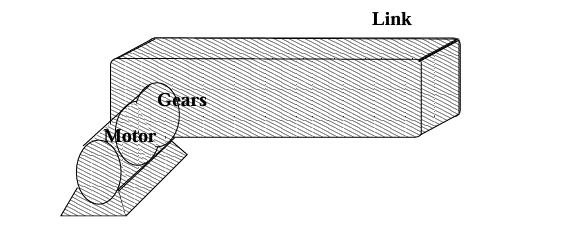
\includegraphics[width=0.6\textwidth]{figs/hw/single_link_robot_arm.png}
    \caption{Single-link robot arm actuated through a geared motor.}
    \label{fig:single_link_robot_arm}
\end{figure}

\noindent Let \(y(t)=\theta(t)\) denote the angular position of the robotic arm. The standard second-order dynamics of the single-link manipulator are as follows:
\begin{equation}
J\ddot{y}+B\dot{y}+Mg\ell\sin(y)=\tau
\label{eq:single_link_second_order}
\end{equation}
where \(J\) is the inertia, \(B\) is the damping coefficient, \(M\) is the mass of the link, \(\ell\) is the distance from the joint to the center of mass, \(g\) is gravity and \(\tau\) is the actuator torque.

\subsection{Extension to a Third-Order Model}

The assignment requires a nonlinear model of order \(n\geq 3\). Therefore, first-order actuator dynamics added:
\begin{equation}
\dot{\tau}=-\alpha \tau + cu
\label{eq:actuator_dynamics}
\end{equation}
where \(u(t)\) is the actuator command input, \(c\) is the input gain, and \(\alpha>0\) represents the actuator time constant effect. Differentiating \eqref{eq:single_link_second_order} gives:
\begin{equation}
J y^{(3)} + B\ddot{y}+Mg\ell\cos(y)\dot{y}=\dot{\tau}
\end{equation}
Substituting \eqref{eq:actuator_dynamics} and using \eqref{eq:single_link_second_order} gives:
\begin{equation}
J y^{(3)}
+
(B+\alpha J)\ddot{y}
+
\alpha B\dot{y}
+
\alpha Mg\ell \sin(y)
+
Mg\ell\cos(y)\dot{y}
=
cu
\label{eq:derived_third_order}
\end{equation}
This equation represents a third-order nonlinear robot arm model, where the nonlinearities originate from the gravity term and from the coupling term \(\cos(y)\dot{y}\).

\subsection{Mathematical Representation}

To match the required structure of the assignment, the robot arm dynamics are represented in the following form:
\begin{equation}
y^{(3)}
+a_1y''
+a_2y'
+b_1(y'')^3
+b_2(y')^3
+b_3\sin(y)
=
cu .
\label{eq:control_oriented_model}
\end{equation}
This model preserves the physical nonlinearities of the robotic arm while satisfying the general nonlinear system structure required. The nonlinear functions are defined as:
\begin{equation}
f_1(y'')=(y'')^3,
\qquad
f_2(y')=(y')^3,
\qquad
f_3(y)=\sin(y).
\end{equation}
The term \(b_3\sin(y)\) represents the nonlinear torque acting on the robotic arm, while the cubic terms \(b_1(y'')^3\) and \(b_2(y')^3\) are used to represent nonlinear actuator and friction effects, respectively. The state variables are defined as:
\begin{equation}
x_1=y,
\qquad
x_2=\dot{y},
\qquad
x_3=\ddot{y}.
\end{equation}
The state vector is therefore given by:
\begin{equation}
x=
\begin{bmatrix}
x_1\\
x_2\\
x_3
\end{bmatrix}.
\end{equation}
Using these state definitions, the system can be written as:
\begin{align}
\dot{x}_1 &= x_2,\\
\dot{x}_2 &= x_3,\\
\dot{x}_3 &=
-a_1x_3
-a_2x_2
-a_3x_1
-b_1x_3^3
-b_2x_2^3
-b_3\sin(x_1)
+cu.
\end{align}

where the system output is:
\begin{equation}
y=x_1.
\end{equation}
The resulting model is a third-order nonlinear single-input single-output (SISO) system that will serve as the basis for following sections.

\bigskip